% !TeX root = ../main.tex

\chapter{系統實作}
本研究已成功實現了系統的核心功能,並在受控的測試環境中進行了全面的概念驗證(Proof of Concept, PoC)。系統的驗證對象包含兩個主要服務,一是遵循微軟AI聊天系統規格\cite{microsoft_ai_chat_protocol}的典型AI聊天服務;二是一個假想的第三方支付服務。用戶可以使用自主身分,在支付費用的前提下使用AI聊天服務。本章將詳細介紹系統的架構和實現細節,並通過流程分析來進一步展現自主身分系統的應用價值。
\section{系統架構}
\begin{figure}
  \centering
  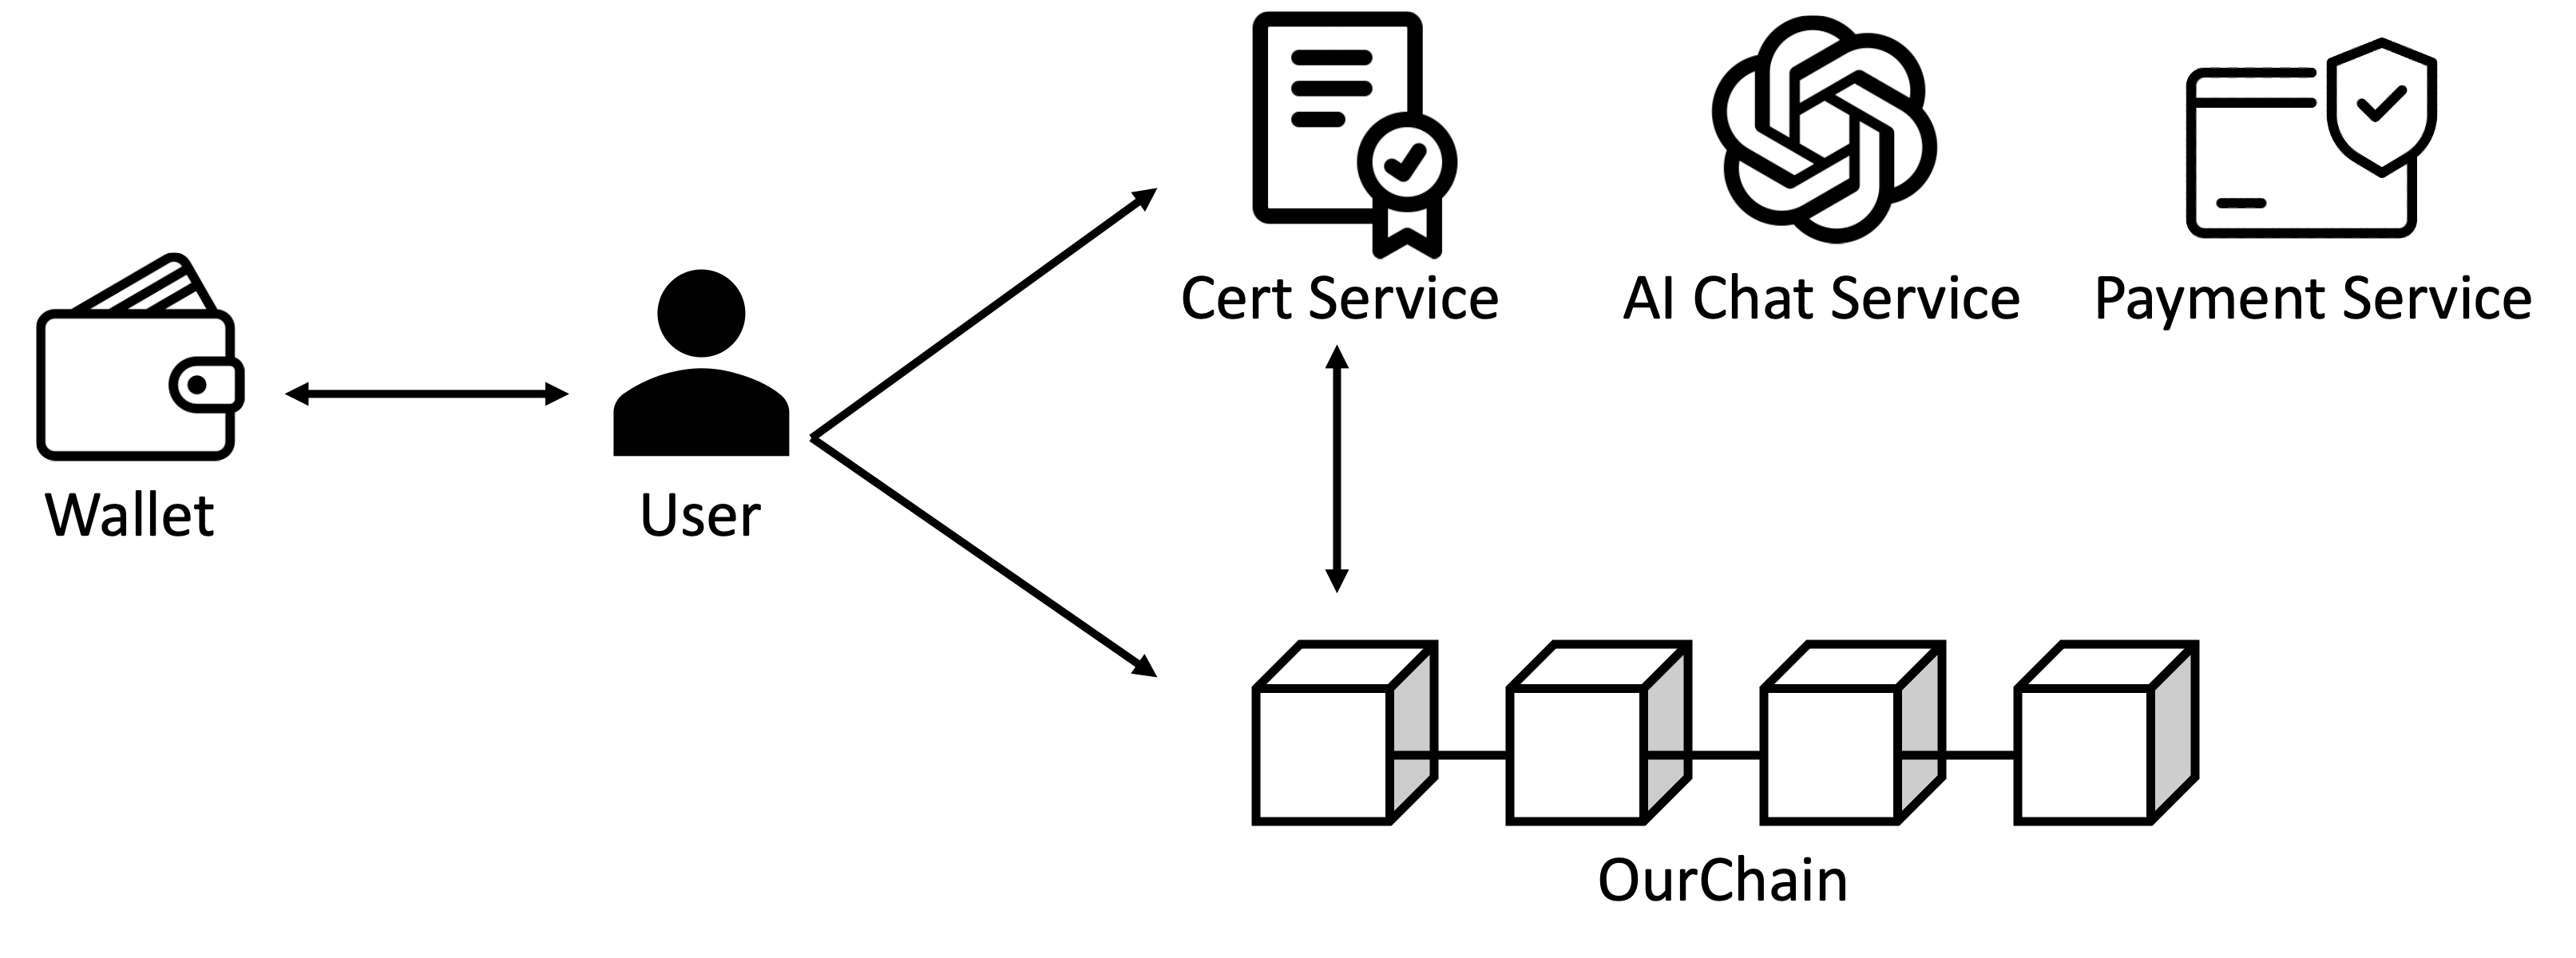
\includegraphics[width=\linewidth, keepaspectratio]{figures/implement.png}
  \caption{AID概念驗證架構簡圖}
  \label{fig:implement}
\end{figure}
整個自主身分系統的概念驗證分成多個模塊如圖\ref{fig:implement},以下按照分層架構來介紹:
\begin{itemize}
  \item \textbf{共識層}: 一條區塊鏈,用於存放「自主證照」和「數據證照」的智能合約。
  \item \textbf{服務層}: 實際與用戶產生互動的服務,包括:
        \begin{itemize}
          \item 一個完成證照所需的簽章服務,用於生成「自主證照」。
          \item 一個AI聊天服務,用於提供AI聊天功能。
          \item 一個支付服務,用於提供AI聊天所需的支付功能。
        \end{itemize}
  \item \textbf{用戶層}: 用戶的手機應用程式,一對一對應到服務層的服務。
\end{itemize}
\section{實現細節}
\begin{table}[htbp]
  \centering
  \caption{系統分層結構及介面}
  \label{tab:system-interfaces}
  \begin{tabularx}{\textwidth}{|l|X|}
    \hline
    \textbf{層次} & \textbf{實現的介面}    \\
    \hline
    共識層         & - 初始化與獲取AID資訊     \\
                & - 設置與獲取證照評論       \\
    \hline
    服務層         & - 簽名證照並上鏈         \\
                & - 驗證證照與管理用戶數據     \\
                & - 點數驗證與證明生成       \\
                & - 登出時數據處理         \\
                & - 身分驗證與登入         \\
                & - 生成與回傳交易證照       \\
    \hline
    用戶層         & - GUI開發 (Flutter) \\
                & - 本地數據存儲 (Hive)   \\
                & - 跨應用數據共享         \\
    \hline
  \end{tabularx}
\end{table}
如\ref{tab:system-interfaces}所示,我們實現了系統的各個層次,並提供了相應的介面。

在共識層中,我們挑選了OurChain\cite{ourlab408_ourchain}作為區塊鏈的實作,並且在其上實現了智能合約。智能合約的介面如下:
\begin{itemize}
  \item \textbf{initAID}: 設置合約的基本資訊,本實作包含擁有者AID和證照簽名。
  \item \textbf{getAIDInfo}: 獲取合約的擁有者AID和證照簽名。
  \item \textbf{setComment}: 設置針對證照的評論,本實作提供純文字紀錄。
  \item \textbf{getComment}: 獲取針對證照的評論。
\end{itemize}
服務層中,我們首先利用Golang調用OurChain的RPC接口來實現智能合約的操作,完成了簽章服務。簽章服務的介面如下:
\begin{itemize}
  \item \textbf{signAID}: 用戶傳入透過「自主證照」生成的明文證照,服務端將其簽名後上鏈,並返回簽名後的證照與合約地址。
\end{itemize}
雖然AI聊天服務和支付服務的具體實現與本研究無直接關係,但我們主要探討如何在這些服務中嵌入自主身分系統。

在AI服務中,使用者必須使用自主身分登入,並擁有足夠的點數才能使用服務。因此我們實作了以下機制:
\begin{itemize}
  \item 驗證並暫存用戶的「自主證照」,實現簡易登入。
  \item 暫存並管理用戶數據(點數、歷史紀錄)。
  \item 要求用戶上傳「數據證照」以驗證點數,並生成新的點數證明。
  \item 登出時回傳用戶數據並清除服務端資料。
\end{itemize}
在支付系統中,我們同樣加入了自主身分系統。其包含以下機制:
\begin{itemize}
  \item 基於「自主證照」進行身分驗證和複雜登入。
  \item 支付後生成「數據證照」作為交易證照。
  \item 不存儲用戶資訊,僅回傳「數據證照」。
\end{itemize}
最後,關於數據層的實現,我們採取了以下措施:
\begin{itemize}
  \item 基於Flutter框架開發跨平台網絡前端應用,為每個服務提供直觀且功能豐富的圖形用戶界面(GUI)
  \item 使用Google開發的Hive套件,以嵌入式資料庫的形式將所有用戶數據存儲在用戶的手機上,確保數據安全
  \item 利用作業系統的剪貼簿共享功能,實現用戶在不同前端應用中輕易共享數據
\end{itemize}
雖然這並不是一個完整的實作,但我們已經成功證明了自主身分系統的可行性,接下來我們將通過流程分析來展示自主身分系統的應用價值。
\section{流程分析}
我們將找出三個典型的用例,配合簡圖與細節流程來展示自主身分系統的應用價值。這三個用例分別是:
\begin{itemize}
  \item 產生新的AID與自主證照
  \item 進入支付服務獲取收據
  \item 使用AI服務對話
\end{itemize}
\subsection{產生新的AID與自主證照}
\begin{figure}
  \centering
  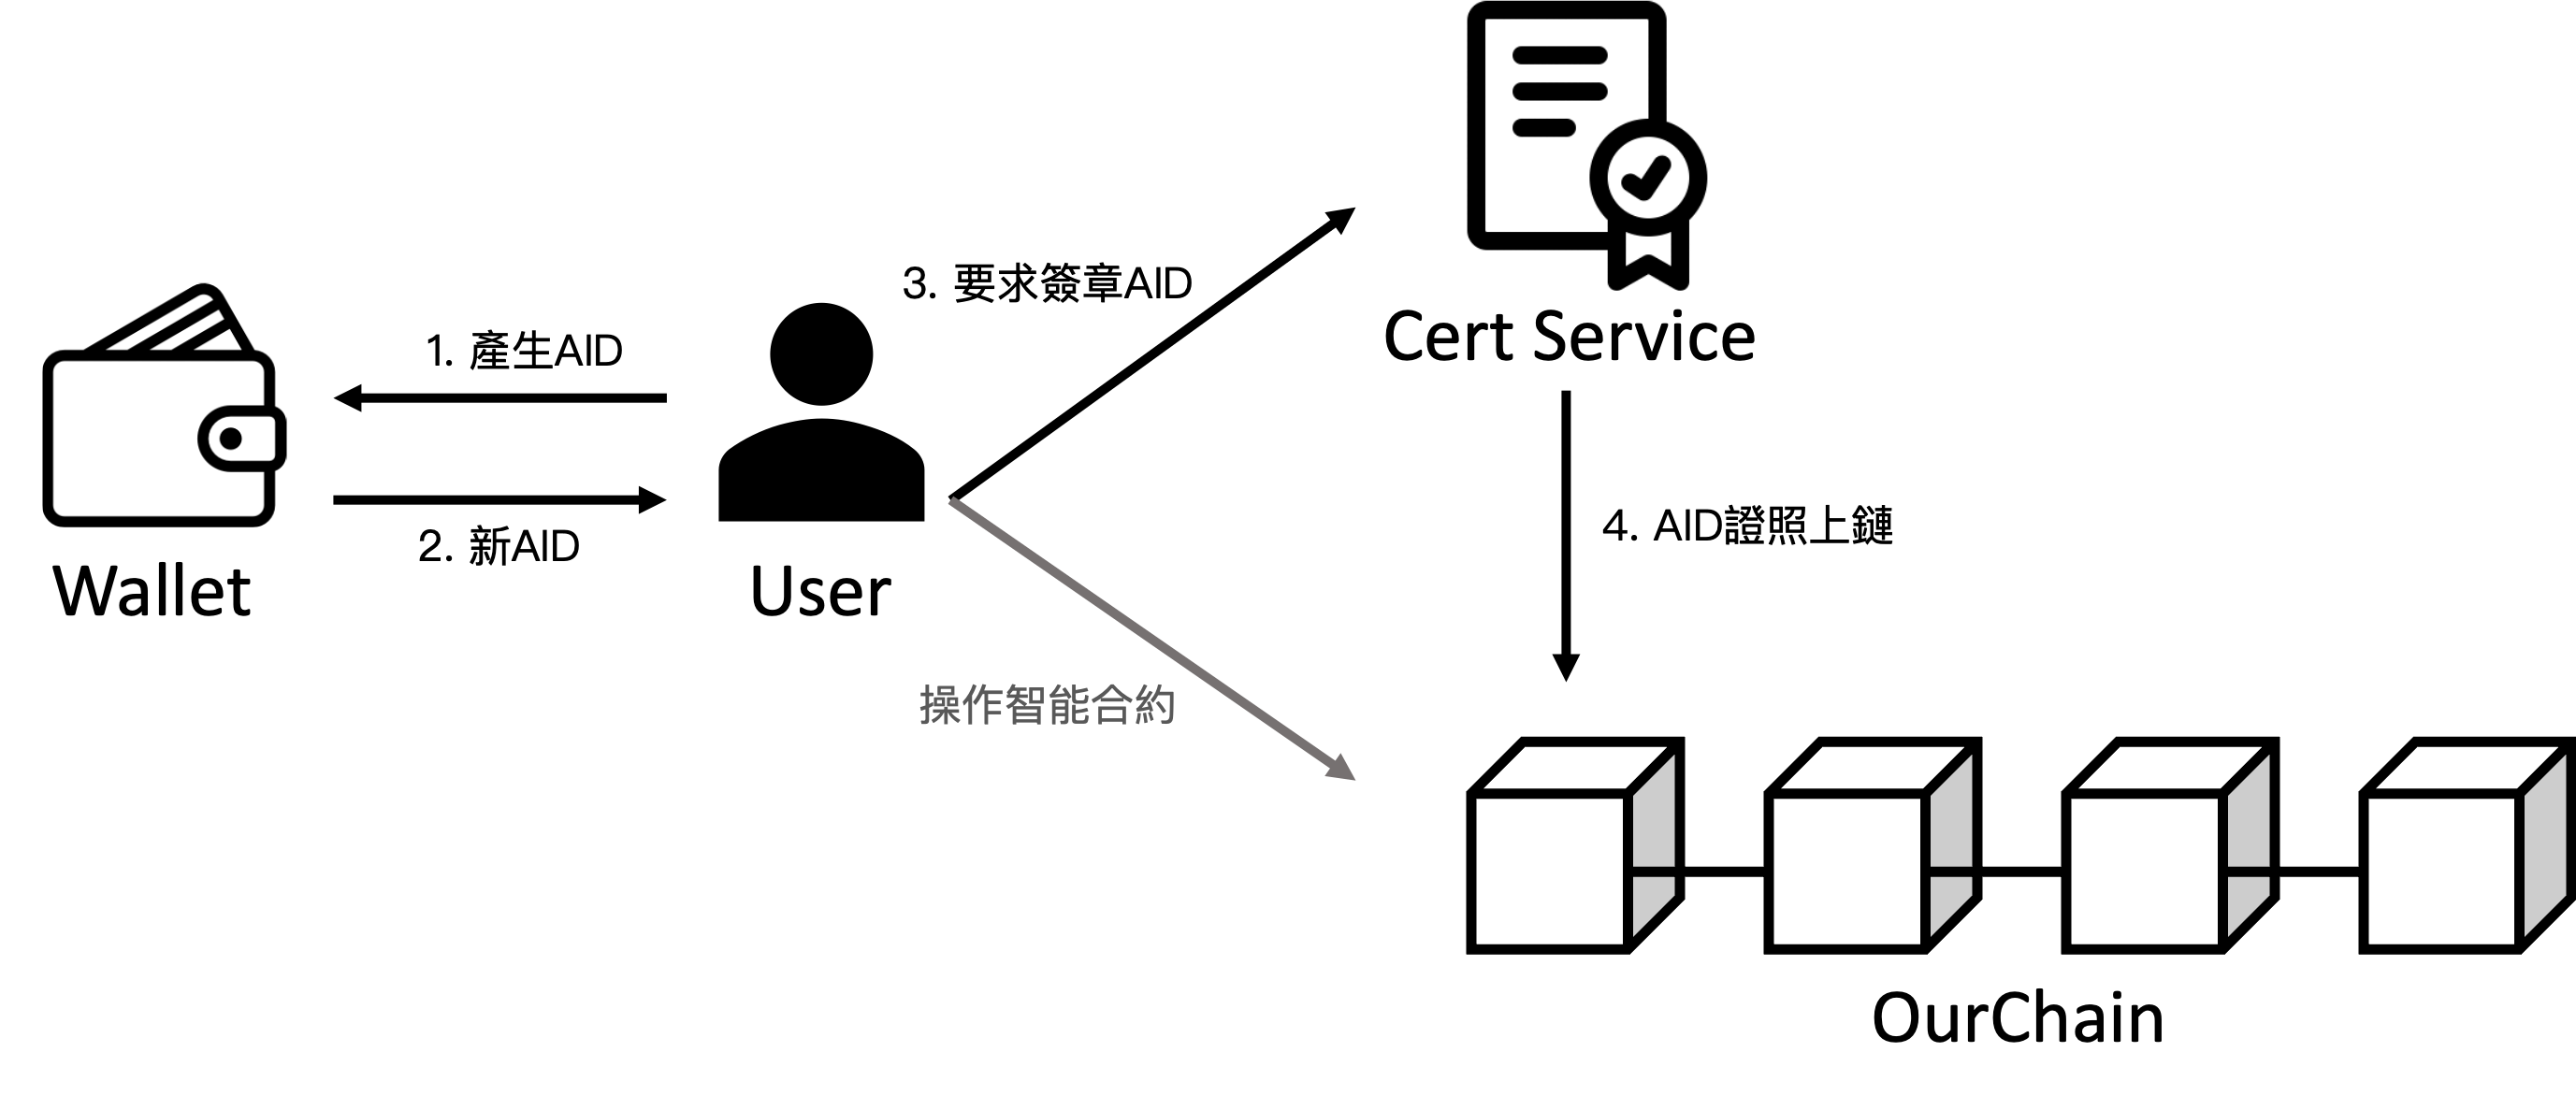
\includegraphics[width=\linewidth, keepaspectratio]{figures/implement-1.png}
  \caption{產生新的AID與自主證照}
  \label{fig:implement-1}
\end{figure}
如圖\ref{fig:implement-1},以下是產生新的AID與自主證照的流程:
\begin{enumerate}
  \item 用戶在任意支援自主身分的前端應用中,點擊「產生新的AID」
        \begin{enumerate}
          \item 在裝置內部基於UUID機制產生唯一識別號後存儲
        \end{enumerate}
  \item 用戶在簽章服務的前端介面中,選擇AID並且點擊「簽章」,產生表單讓用戶填寫資料
  \item 用戶填寫個人資訊,包含別名與pin碼,並且點擊「確認」
        \begin{enumerate}
          \item 透過用戶填入的資訊與AID中的識別號,生成未簽名「自主證照」
          \item 把自主證照傳入服務層產生簽名並上鏈
          \item 服務端回傳簽名後的「自主證照」與合約地址,用戶存儲在個人設備
        \end{enumerate}
\end{enumerate}
通過這樣的流程,用戶自主的生成了自己的AID和自主證照,整個用戶識別不依賴單一服務商,而是由用戶自己控制。
\subsection{進入支付服務獲取收據}
\begin{figure}
  \centering
  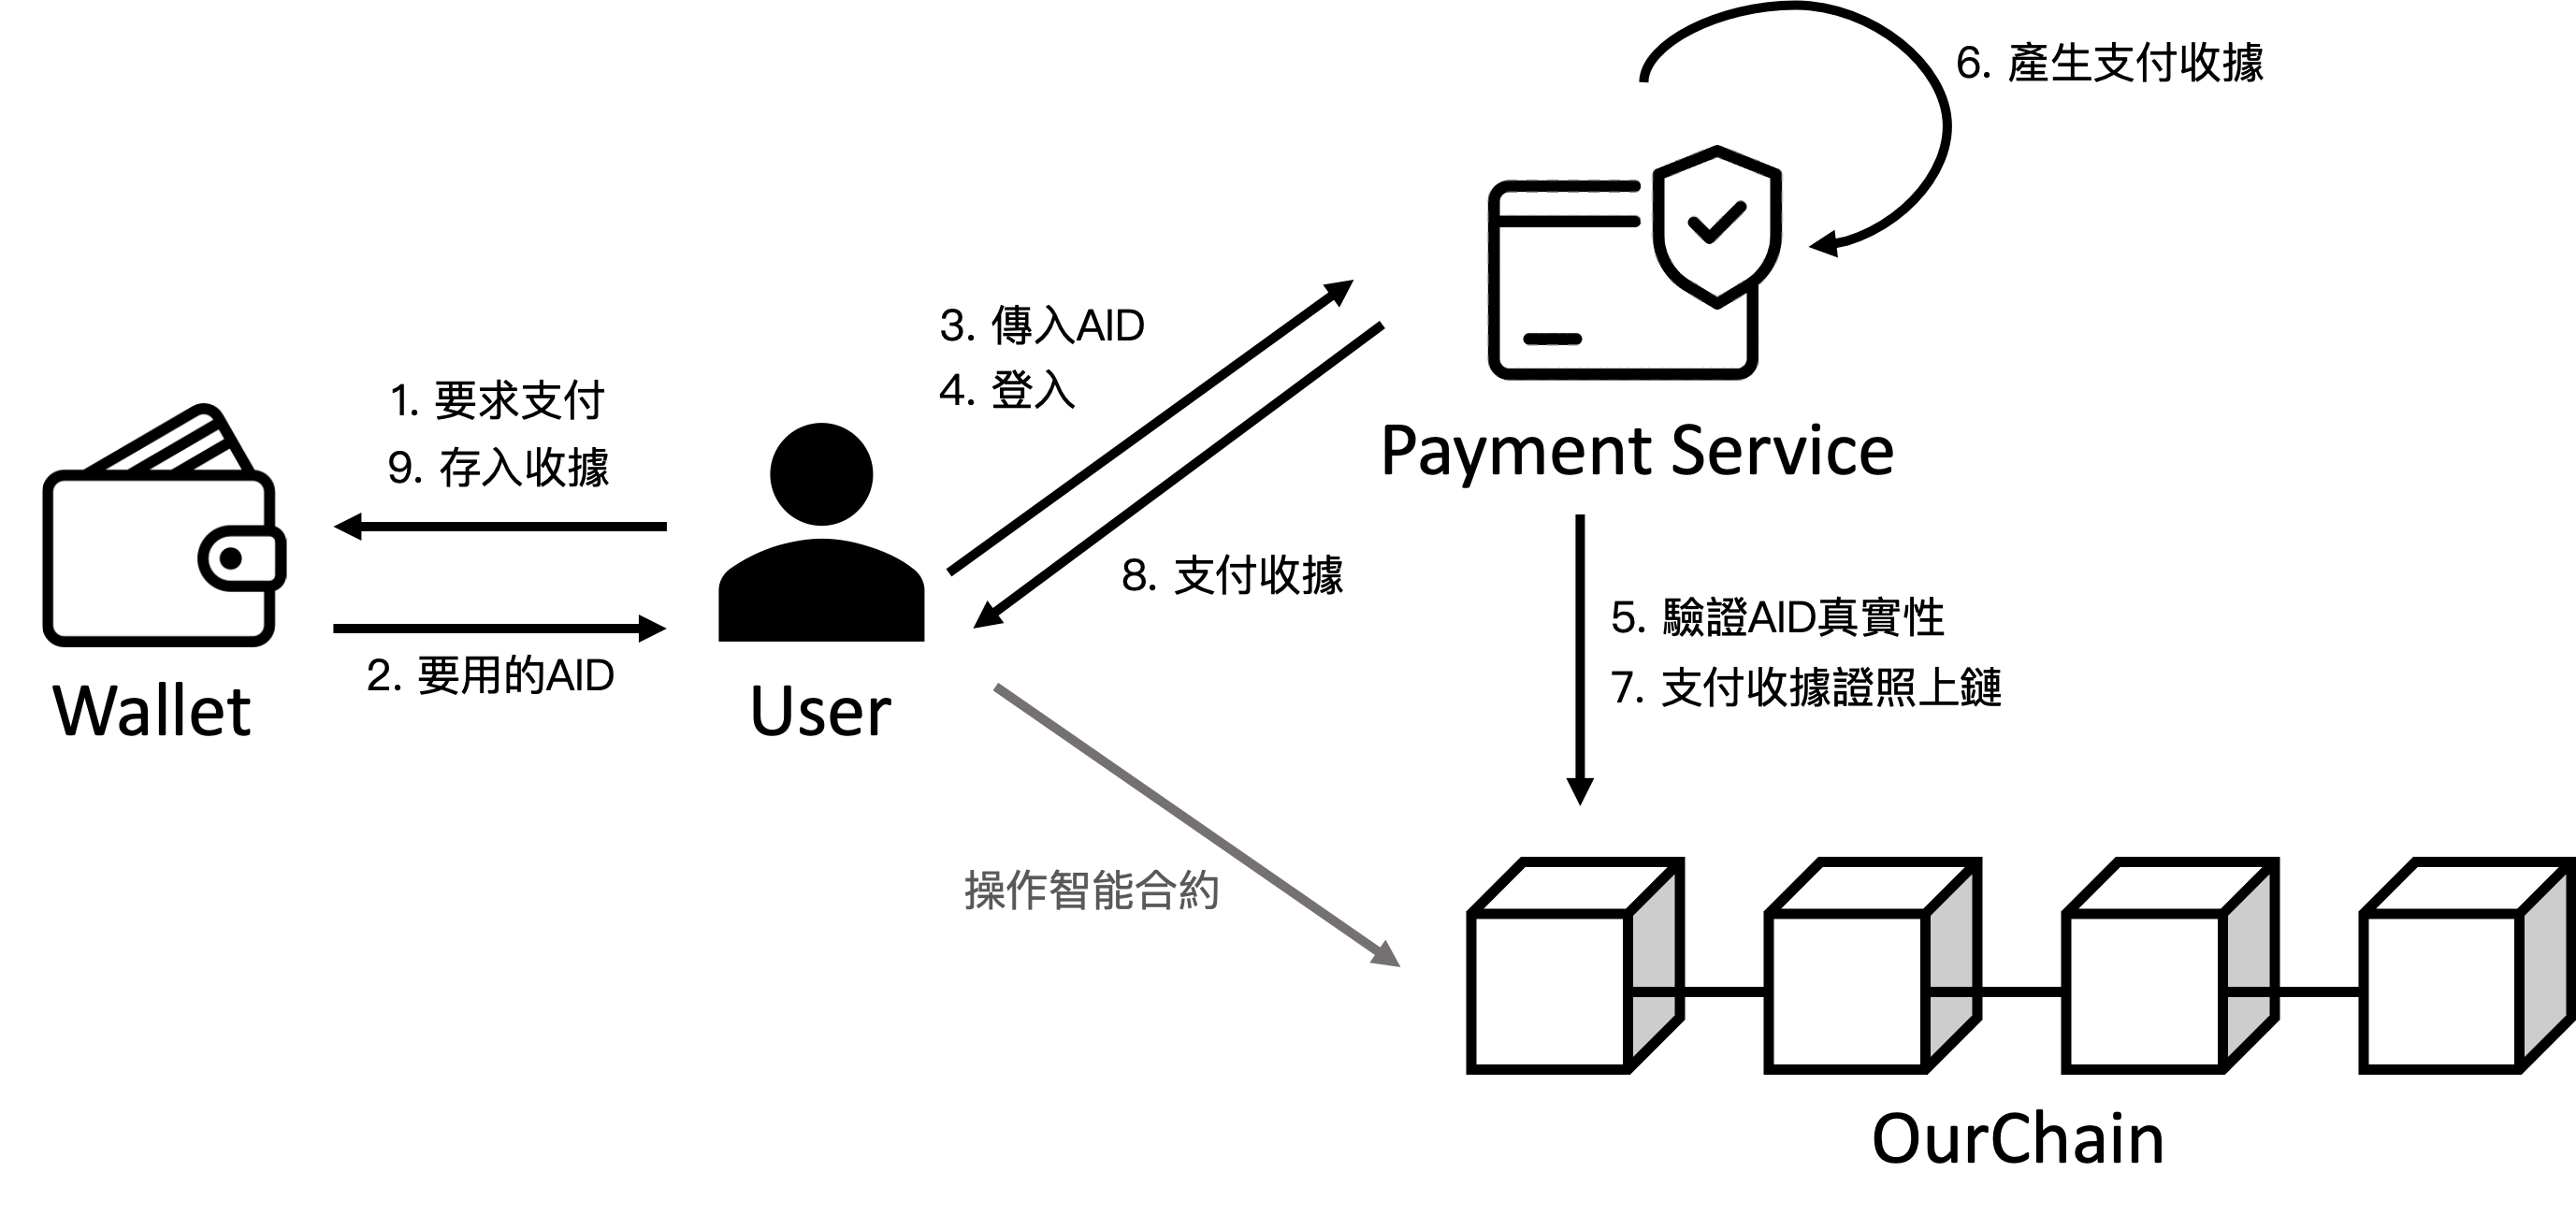
\includegraphics[width=\linewidth, keepaspectratio]{figures/implement-2.png}
  \caption{進入支付服務獲取收據}
  \label{fig:implement-2}
\end{figure}
如圖\ref{fig:implement-2},以下是進入支付服務獲取收據的流程:
\begin{enumerate}
  \item 用戶在支付服務的前端介面中,選擇AID並且點擊「支付」
        \begin{enumerate}
          \item 自動取用設備上存放的「自主證照」,上傳至服務端,觸發複雜登入
          \item 數據層的前端介面自動取用設備上的私鑰產生簽章完成登入
          \item 服務端驗證簽章後,完成支付,於是生成「數據證照」並上鏈
          \item 服務端回傳「數據證照」給用戶存儲在個人設備
        \end{enumerate}
  \item 用戶在支付服務的前端介面中,點擊「查看收據」
\end{enumerate}
通過這樣的流程,用戶可以在支付後獲取到一份「數據證照」,作為交易的證照,用戶可以在任何時候查看這份證照,而不需要依賴支付服務商。
\subsection{使用AI服務對話}
\begin{figure}
  \centering
  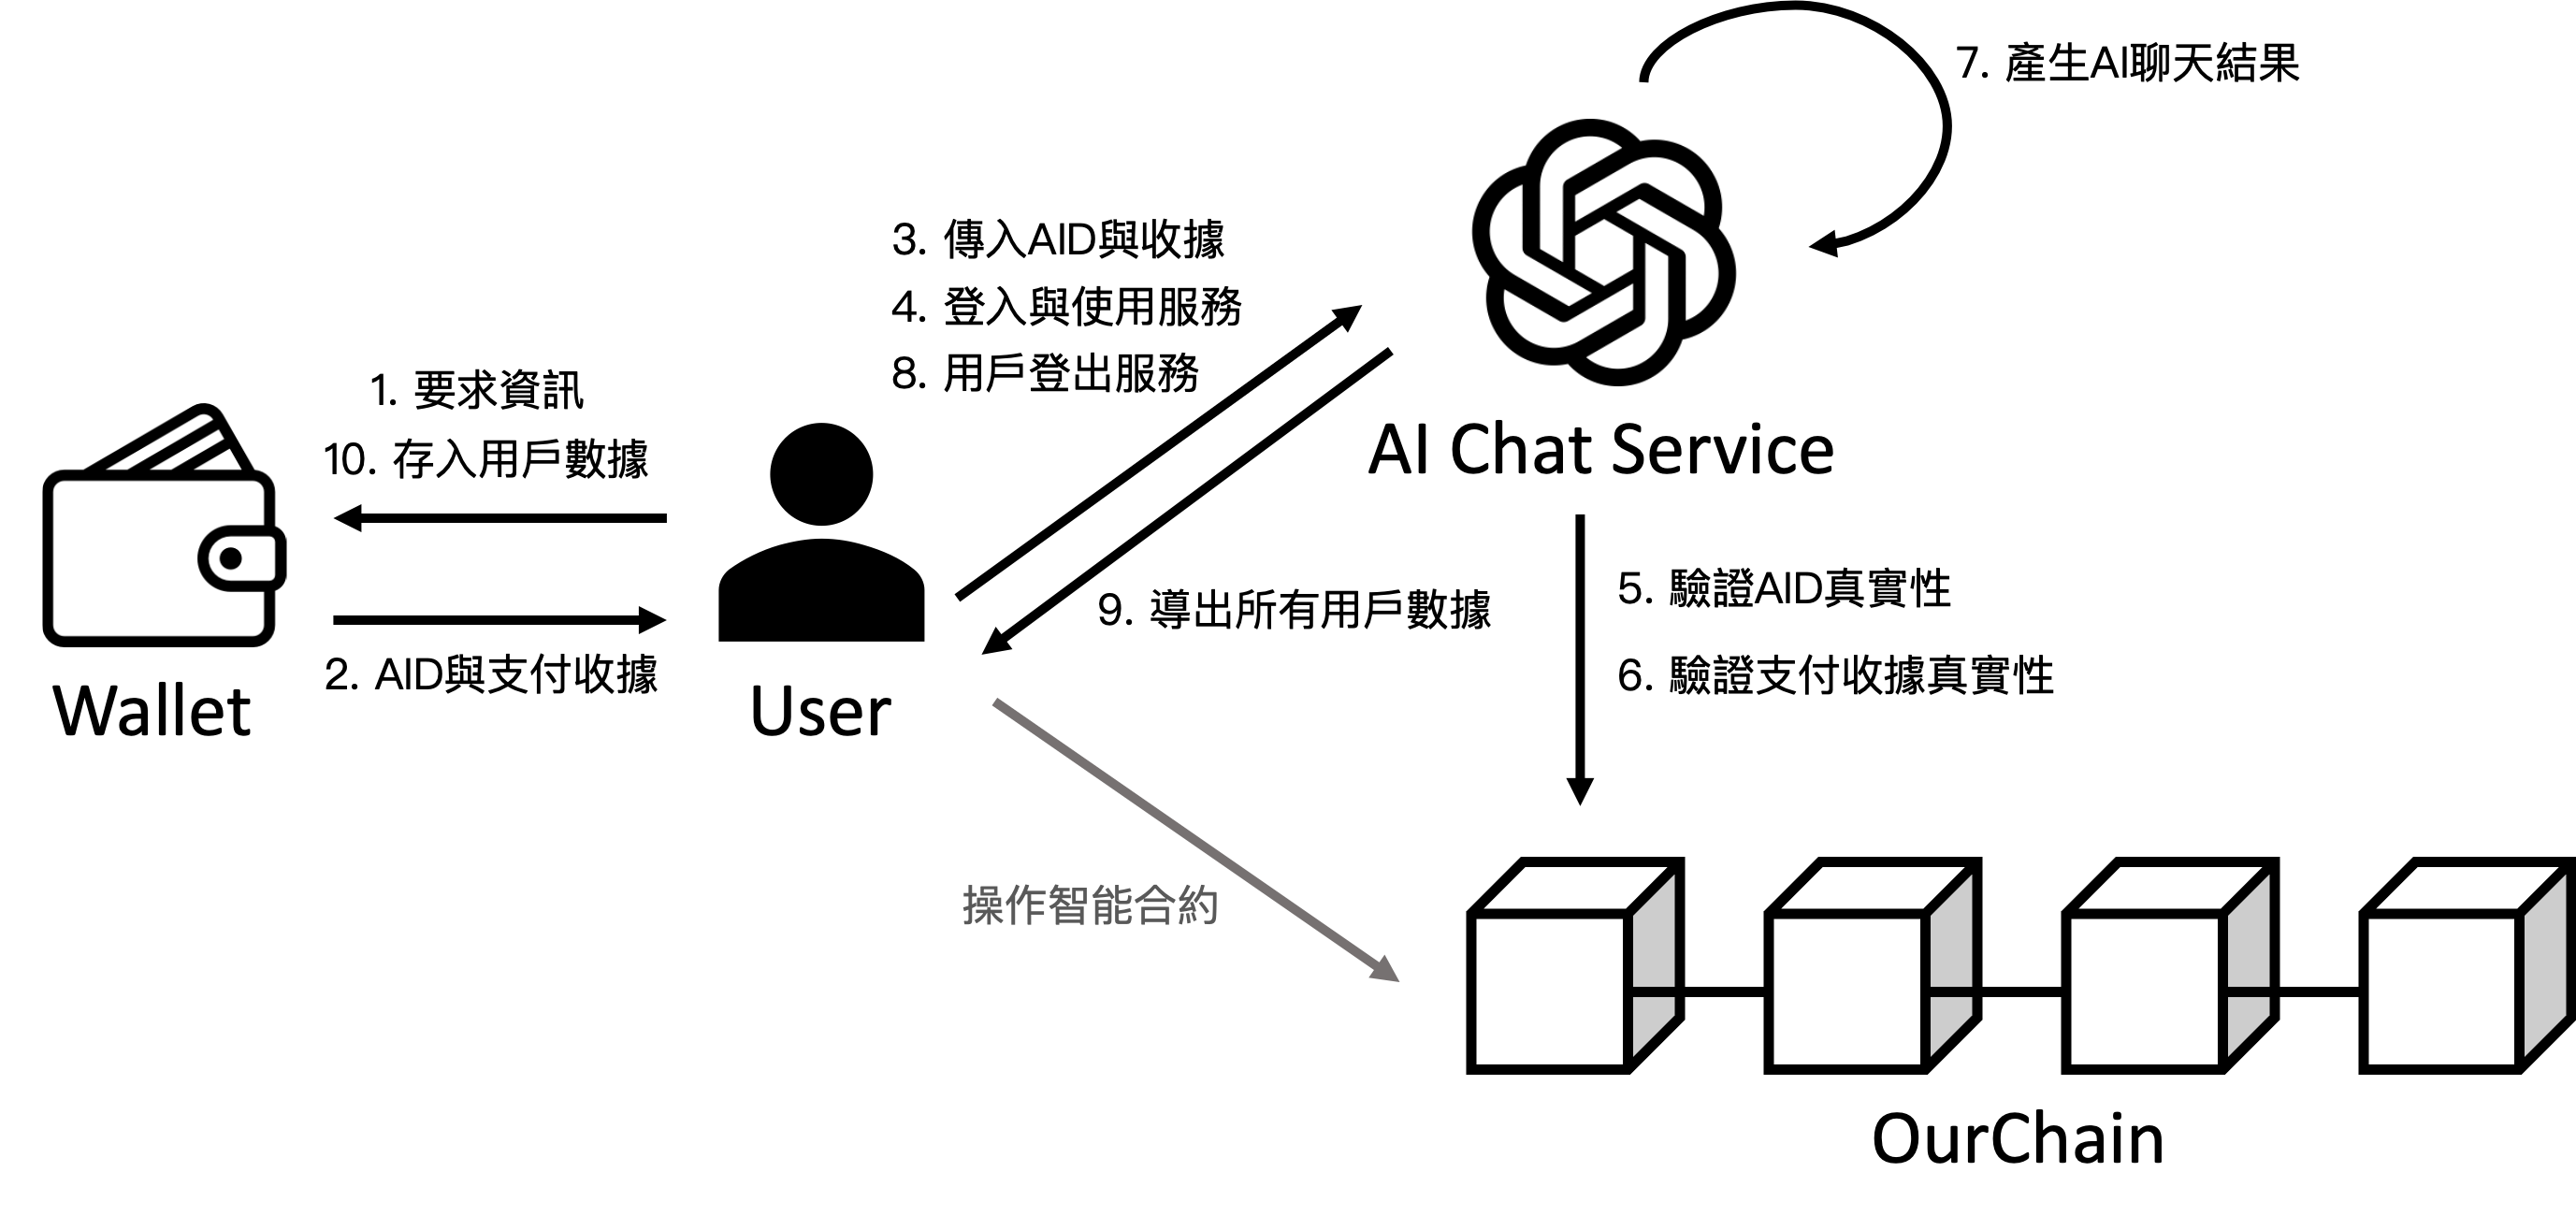
\includegraphics[width=\linewidth, keepaspectratio]{figures/implement-3.png}
  \caption{產生新的AID與自主證照}
  \label{fig:implement-3}
\end{figure}
如圖\ref{fig:implement-3},以下是使用AI服務對話的流程:
\begin{enumerate}
  \item \textbf{登入}:
        \begin{enumerate}
          \item 使用者進入AI服務的前端介面
          \item 傳入選定AID的「自主證照」,觸發簡易登入
          \item 用戶使用證照上的別名與密碼登入
          \item 登入後即開始AI服務中的一次對話
        \end{enumerate}
  \item \textbf{對話前}:
        \begin{enumerate}
          \item AI服務接受數據層中上傳的用戶點數與歷史數據
          \item 要求用戶上傳點數的「數據證照」,以確保點數真實性
        \end{enumerate}
  \item \textbf{對話中}:
        \begin{enumerate}
          \item 用戶與AI進行對話
          \item 每次對話結束後,AI服務更新暫存的用戶點數與歷史數據
          \item 用戶即便離開對話,也只需使用別名與密碼簡易登入即可繼續,無需重新上傳數據
        \end{enumerate}
  \item \textbf{登出}:
        \begin{enumerate}
          \item 用戶選擇離開系統
          \item AI服務將用戶點數、歷史數據與相關「數據證照」回傳至個人裝置
          \item 系統刪除所有用戶數據
        \end{enumerate}
\end{enumerate}
通過這樣的流程,我們實現了數據與服務分離的目標,讓用戶能夠更加方便地管理自己的數據。
\section{本章小結}
儘管本實現並非完整的商業系統,但已成功證明了自主身分系統的可行性和潛在價值。透過在AI聊天服務、支付系統等實際場景中的應用,展現了該系統在提升使用者隱私、資料安全和身分管理方面的巨大潛力。未來研究可進一步探討該系統在更廣泛領域的應用,以及在大規模商業環境中的實施策略。